\newpage
\chapter{Systems Analysis and Design}

1. Specific Requirements\\
a. Need searches based on his interests\\
b. user needs to save a lot of time from this system\\

2. External Interface Requirements\\
a. Allow user to search for his query\\
b. Selection of the type of algorithm to be used.\\
c. Show a list of results or fetched URLs based on his interest\\
d. Redirection to the clicked URLe from this system\\

3. Functional Requirements\\
This project supports all types of browsers. We are using simple questionnaires to
understand the user experience over a particular website.
The major software requirements from the deployer side are –\\
1) Python IDE\\
2) Web Browser (Chrome, Edge etc)\\
3) Legal Website to scrape data\\
4) Web Scraping Tool (Parsehub)\\

4. Performance Requirement\\
This provides a highly Personalised result to its users due to use of page rank algorithm and
Pseudo Relevance Feedback. If there is extensive damage to a wide portion of the database
due to catastrophic failure the recovery method restores a past copy of the database that
was backed up to archival storage and reconstructs a more current state by reapplying or
redoing the operations of committed transactions from the backed up log, up to the time of
failure.\\

\section{System Designing/Modeling}
Module 1 - Collection of data ( by web scraping ) - Web Scraping (also termed Screen
Scraping, Web Data Extraction, Web Harvesting etc.) is a technique employed to
extract large amounts of data from websites\\
1. We can gather information depending on three approaches:\\
a. Information gathering approach(whether implicit/explicit)\\
b. Type of information(users and their usage behavior when interacting with the system)\\
b. Source of information(gathered at the server-side or at the client-side)\\
2. In the implicit method, information is gathered unobtrusively, without any effort from the
user.\\
3. In the explicit method, the users themselves have to explicitly supply information to the
system, whether positive or negative.\\
Module 2 -Analysing and pre-processing the data -\\
1. Finding the missing values.\\
2. Finding out inconsistent data.\\
3. Dealing with Duplicate values.\\
4. Data Transformation\\
5. Data Reduction\\
Module 3 - Personalization in PIR systems is generally performed by adapting the query
and/or the results. Query adaptation: Query adaptation attempts to expand the terms of
the user’s query with other terms, with the aim of retrieving more relevant results.\\
1. processing the user model\\
2. processing aggregate usage information\\
3. pseudo-relevance feedback\\
4. global analysis\\
5. Explicit relevance feedback\\
6. interactive query expansion\\
Module 4 - Applying the suitable and most appropriate algorithm so that we could get more
relevant and personalized results.\\

\section{System Architecture}
The major functions that product must perform are:\\
1. Scraping of data\\
Scraping is the process of collecting structured web data in an automated fashion. It’s
also called web data extraction. Some of the main use cases of web scraping include
price monitoring, price intelligence, news monitoring, lead generation and market
research among many others\\
2. Analyzing and preprocessing the data\\
Data analyzing is a process of inspecting, cleansing, transforming and modeling data
with the goal of discovering useful information, informing conclusions and supporting
decision-making. Data analysis has multiple facets and approaches, encompassing
diverse techniques under a variety of names, and is used in different business, science,
and social science domains. In today’s business world, data analysis plays a role in
making decisions more scientific and helping businesses operate more effectively.\\
3. Classification to show specific results to the users\\
The searched product will be categorised and classified according to the users need
and accordingly results will be displayed\\
4. Applying Algorithm\\
Suitable algorithm will be used in order to enhance the system performance.\\
5. Speech Recognition\\
We are adding voice assistance to it, in order to make it more user friendly .As we
know Python is a suitable language for script writers and developers.The query for
the assistant can be manipulated as per the user’s need.

\subsection{System Architecture}


\begin{figure}[h!]
    \begin{center}
        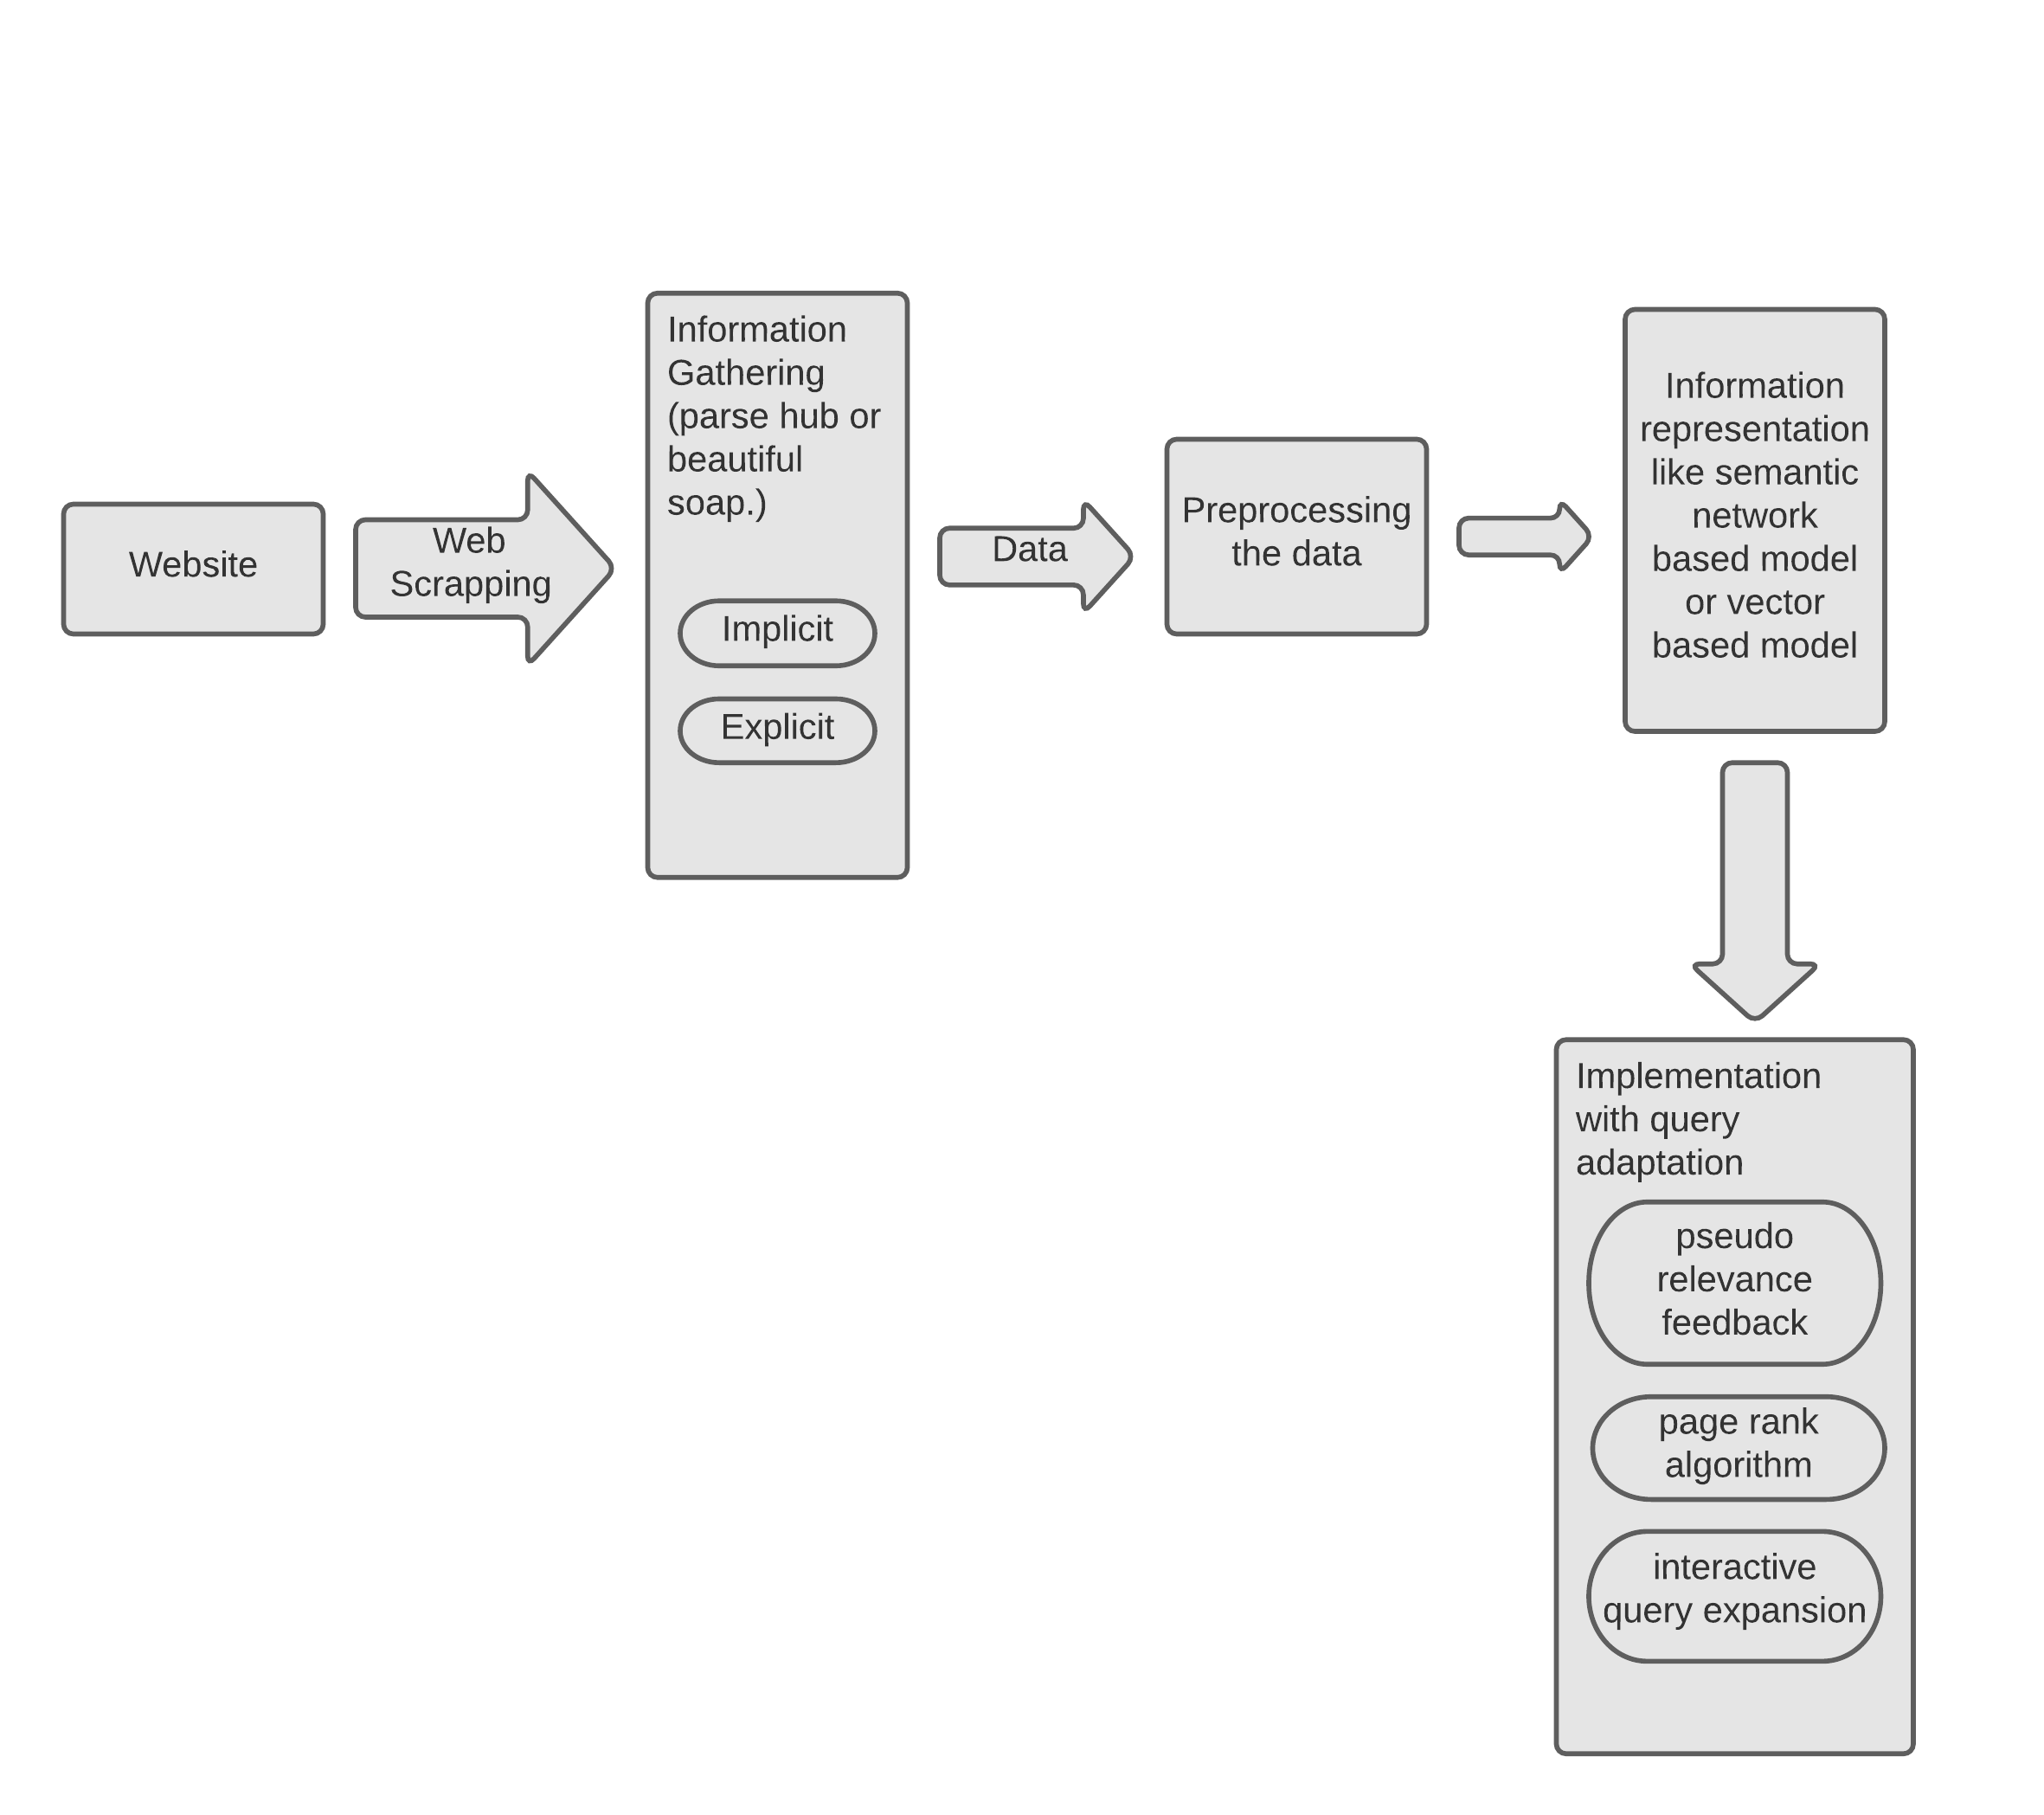
\includegraphics[scale=0.25]{sys}
        \caption{System Design}
    \end{center}
\end{figure}


\begin{figure}[h!]
    \begin{center}
        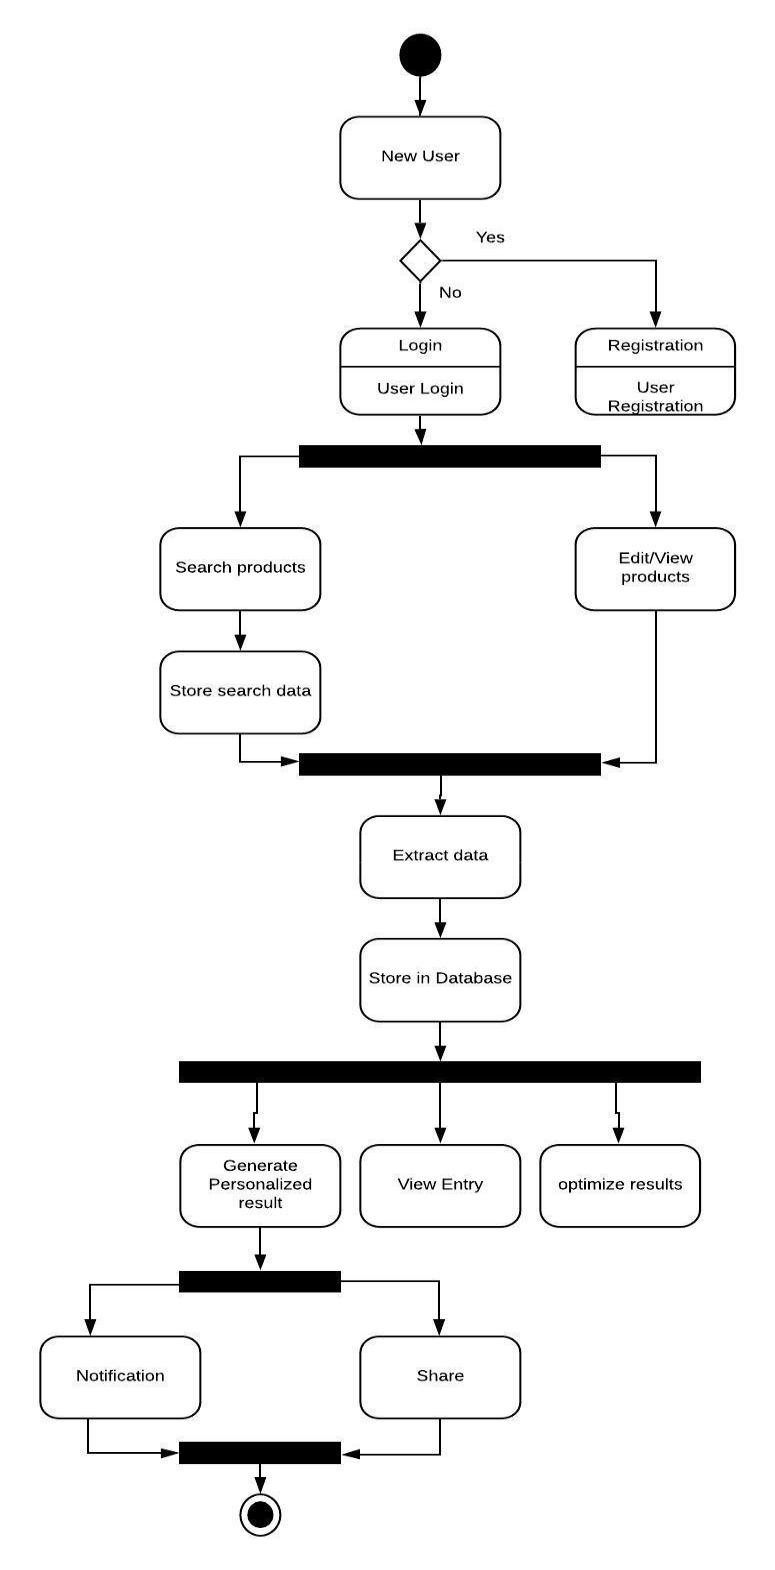
\includegraphics[scale=0.6]{stated}
        \caption{State Diagram}
    \end{center}
\end{figure}

\begin{figure}[h!]
    \begin{center}
        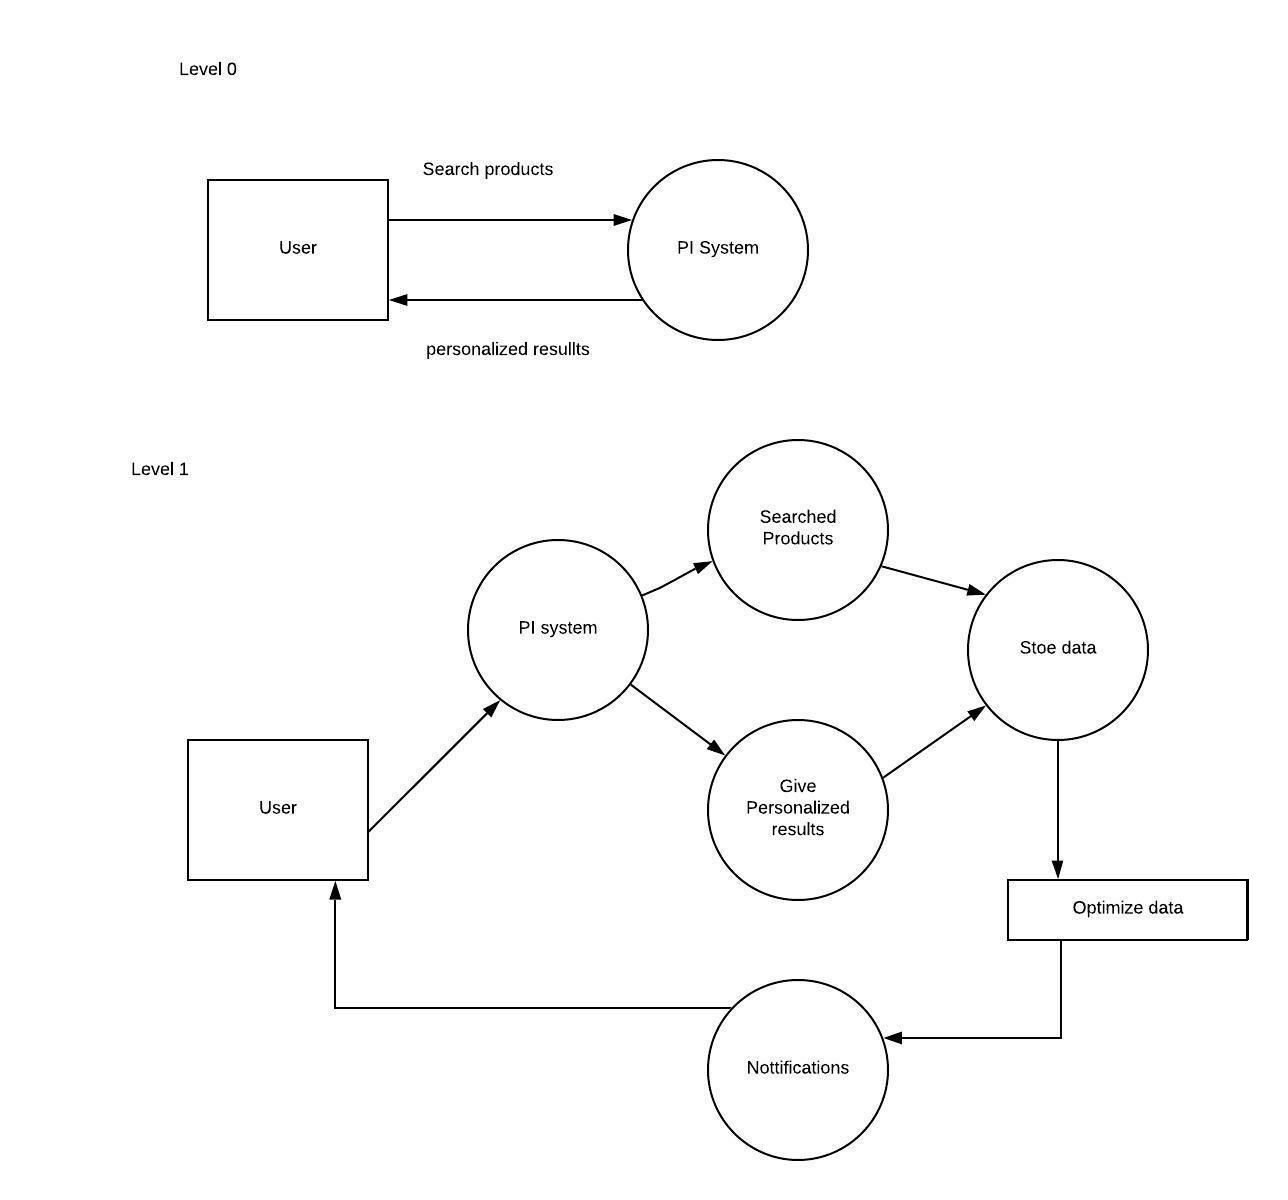
\includegraphics[scale=0.45]{dfdd}
        \caption{DFD Diagram}
    \end{center}
\end{figure}

\begin{figure}[h!]
    \begin{center}
        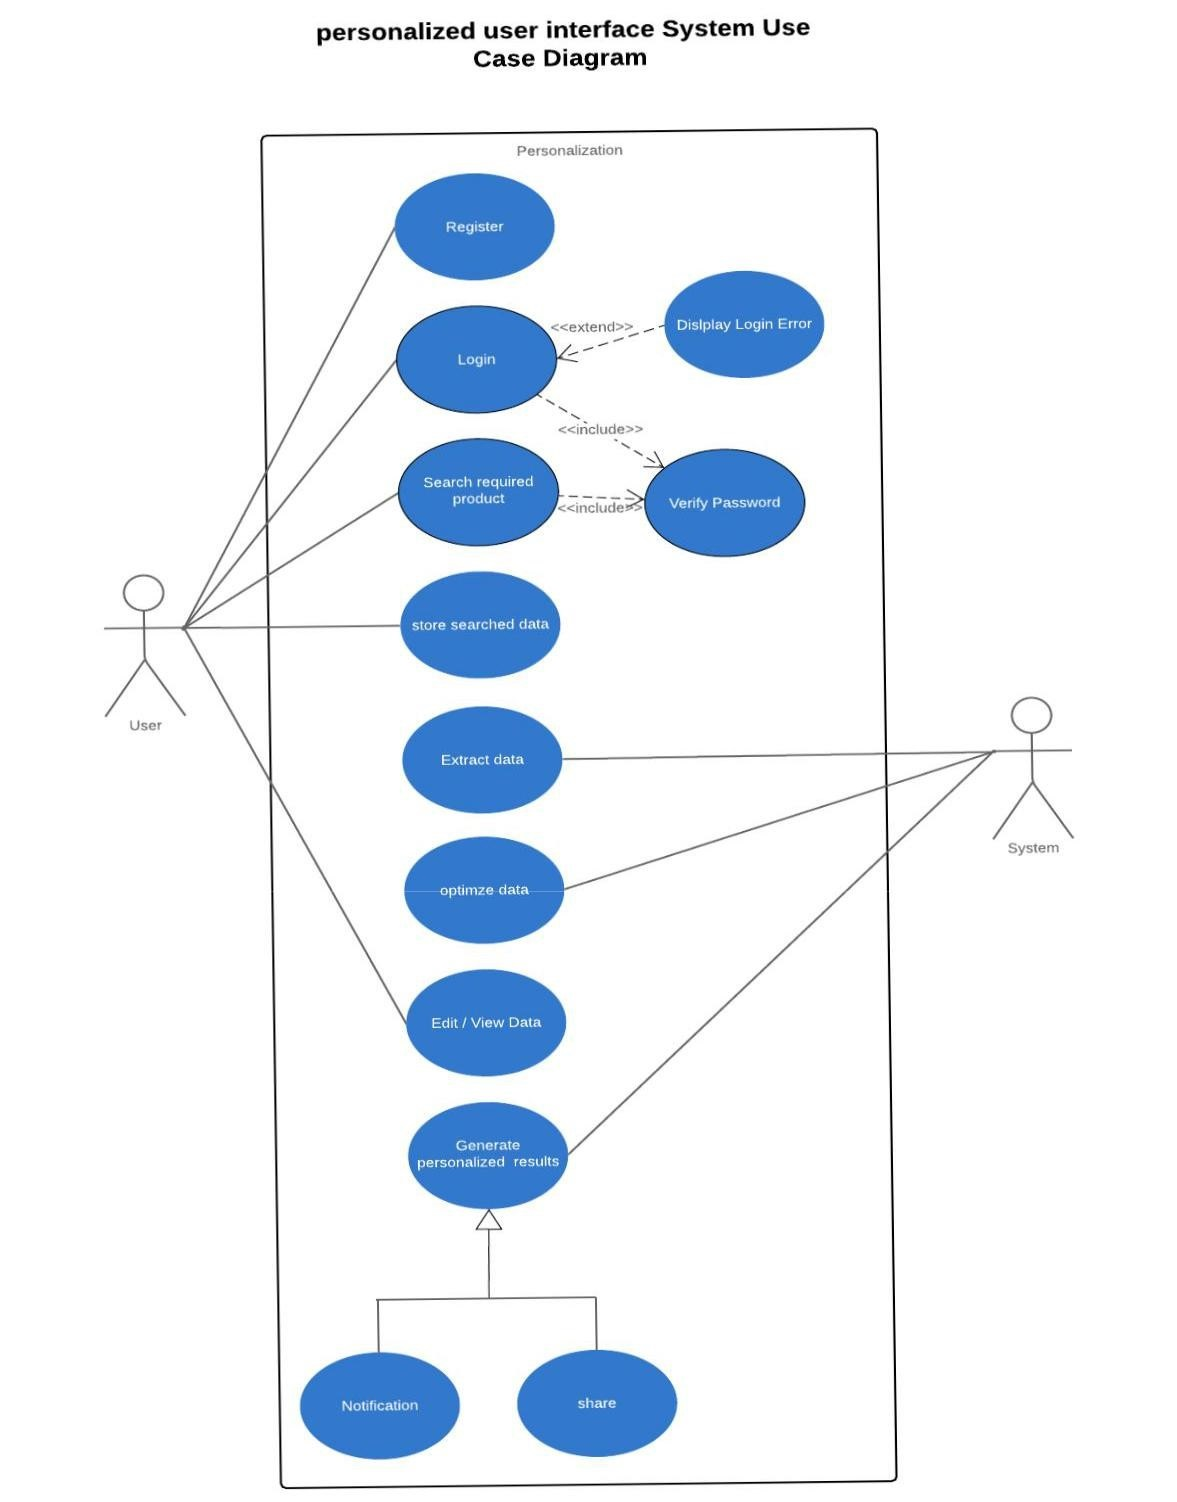
\includegraphics[scale=0.6]{used}
        \caption{Use Case Diagram}
    \end{center}
\end{figure}
\vspace{10mm}
\hrule
